\chapter{Referencial Teórico}
\section{Sobre as Seções de Choque Diferencial e Total}
Neste trabalho iremos tratar do método dos fótons equivalentes. O problema de
interesse deste método é o do cálculo da seção de choque em processos de
colisão ou de produção de partículas. Por seção de choque consideramos como uma
quantidade experimental de interesse em colisões \cite{griffiths_particle}.
Inicialmente, discutindo sob uma lente clássica, podemos considerar um processo
de espalhamento, no qual a partícula entra na região de influência do centro de
potencial, o qual possui parâmetro de impacto $b$, conforme a Figura
\ref{cross_section_def}. A partir da geometria apresentada, podemos obter os
seguintes diferenciais de área e ângulo sólido, respectivamente,
\begin{gather}
d\sigma = |b\, db\, d\phi|,\\
d\Omega = |\sen \theta \, d\theta \, d\phi|.
\end{gather}
Assim, a razão entre as duas é escrita como,
\begin{equation}
\frac{d\sigma}{d\Omega} = \bigg| \frac{b}{\sen \theta} \frac{db}{d\theta}
\bigg|. \label{diff_cross_section}
\end{equation}
Aqui, assumimos que o potencial do centro de espalhamento tem simetria
azimutal, em $\phi$.

A quantidade dada na equação (\ref{diff_cross_section}) é denominada de seção
de choque diferencial \cite{griffiths_particle}.  A seção de choque total
será a seção de choque diferencial integrada sobre todo o ângulo sólido
$\Omega$ sendo ela dada por,
\begin{equation}
\sigma = \int \frac{d\sigma}{d\Omega} \sen \theta \, d\theta \, d\phi .
\end{equation}

\begin{figure}[h]
\centering
	\captionsetup{width=\textwidth}
	\caption{Área diferencial $d\sigma$ indicada com centro de espalhamento
	estático com parâmetro de impacto $b$. A partícula é espalhada em um
	elemento diferencial de ângulo sólido $d\Omega$.}
\label{cross_section_def}
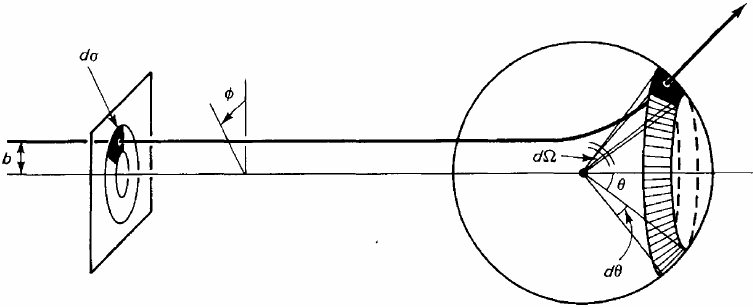
\includegraphics[width=\textwidth]{./figs/cross_section.jpeg}
\fonte{Retirado de \cite{griffiths_particle}}
\end{figure}

Agora, vamos considerar um feixe de $N$ partículas monoenergéticas (de mesma
energia), todas sendo lançadas contra um dado centro de espalhamento. A
luminosidade $\mathcal{L}$ é definida como a quantidade de partícula que
atravessam a região de espalhamento por unidade de área e unidade de tempo.
Assim, a quantidade de partículas que atravessam a área $d\sigma$ por unidade
de tempo é dada por,
\begin{equation}
	dN = \mathcal{L} d\sigma.
\end{equation}
Disso segue que,
\begin{equation}
	\frac{d\sigma}{d\Omega} = \frac{1}{\mathcal{L}} \frac{dN}{d\Omega}.
\end{equation}
Essa acaba sendo uma maneira mais útil de escrevermos a seção de choque
diferencial. Sendo assim, o número de partículas espalhadas em um ângulo sólido
$dN$ dividido por $d\Omega$ e pela luminosidade.


\section{Derivação do Método dos Fótons Equivalentes}
Vamos tomar uma partícula pontual eletricamente carregada viajando a
velocidades relativísticas perto de um alvo, que iremos considerar como fixo. A
interação desta com o alvo se dará pelos campos gerados pela partícula, uma vez
que o movimento desta consiste em uma variação da carga no espaço. Essa
interação entre a partícula incidente e o alvo consiste em uma perturbação do
alvo e no espalhamento da partícula incidente.  O estudo desses campos é de
interesse pois, assim, podemos obter o número de fótons equivalentes desses
campos\footnote{Aqui fazemos a obtenção dos fótons a partir de uma perspectiva
semi-clássica.}. Com o uso do número de fótons equivalentes é possível o estudo
de processos atômicos e subatômicos, dos quais podemos obter seções de choque
de interesse.

O método dos fótons equivalentes aqui discutido consiste em aproximar os campos
produzidos por cargas carregadas em movimento por pulsos de ondas.  Através de
uma transformada de Fourier desses campos, obtemos o espectro de frequência dos
campos e, consequentemente, o número de fótons equivalentes destes, que pode
ser usado para calcular seções de choque de interesse.  Além disso, aqui e no
resto do trabalho usamos unidades naturais ($\hslash = c = 1$) com unidades de
Heaviside-Lorentz \cite{jackson3} \cite{mariola} \cite{caruso_quanta}
\cite{nivaldo_cap6}.

Vamos calcular como os campos elétrico ($\vec{E}$) e magnético ($\vec{B}$) de
uma partícula carregada com carga $q$ são percebidos quando esta passa na
vizinhança de um ponto de observação $P$, como indicado na Figura
\ref{fig_charge-passing}. Vamos tomar $\Sigma '$ como o referencial solidário à
partícula carregada e $\Sigma$ como o referencial solidário ao ponto $P$,
assumindo que a origem dos sistemas dos referenciais coincidam no tempo
$t=t'=0$. Com isso, lembramos que os campos em termos dos potenciais escalar
$\Phi$ e vetor $\vec{A}$ são,
\begin{gather}
	\vec{E} = - \nabla \Phi - \frac{\partial \vec{A}}{\partial t}, \\
	\vec{B} = \nabla \times \vec{A}.
\end{gather}
Com isso, é mais fácil calcularmos a transformação dos campos a partir do
tensor eletromagnético $F^{\mu \nu}$ (onde usamos a notação de
Einstein\footnote{A notação de soma de Einstein implica que estamos somando os
índices repetidos indo de 0 a 3. Por exemplo, isso implica que $x^\mu y_\mu =
x^0 y_0 + x^1 y_1 + x^2 y_2 + x^3 y_3$.}), cujas componentes são dadas pela
matriz,
\begin{equation}
    (F^{\mu \nu}) = \begin{pmatrix}
		0 & -E_1 & -E_2 & -E_3 \\
		E_1 & 0 & -B_3 & B_2 \\
		E_2 & B_3 & 0 & -B_1 \\
		E_3 & -B_2 & B_1 & 0
	\end{pmatrix}.
\end{equation}
Assim, a transformação das componentes pode ser dada por
\begin{equation}
    {F'}^{\mu \nu} = \frac{\partial {x'}^\mu}{\partial x^ \alpha}
    \frac{\partial {x'}^\nu}{\partial x^\beta}F^{\alpha \beta} = \Lambda ^\mu
    _\alpha \Lambda ^\nu _\beta F^{\alpha \beta},
    \label{eq_tensor_trans}
\end{equation}
onde $\Lambda ^\mu _\nu$ são as componentes da matriz de transformação de
Lorentz \cite{nivaldo_cap6}. Para o caso de um impulso na direção $x$, como
estamos considerando, esta será,
\begin{equation}
	(\Lambda ^\mu _\nu) = \begin{pmatrix}
		\gamma & -\gamma \beta & 0 & 0 \\
		-\gamma \beta & \gamma & 0 & 0 \\
		0 & 0 & 1 & 0 \\
		0 & 0 & 0 & 1
	\end{pmatrix},
\end{equation}
onde $\gamma = (1-\beta ^2)^{-1/2}$ e $\beta = v/c$ são os parâmetros
relativísticos. Calculando os termos não nulos a partir da expressão
(\ref{eq_tensor_trans}), obtemos as seguintes componentes dos campos elétrico e
magnético, respectivamente,
\begin{equation}
	\label{eq_field_trans}
    \begin{cases}
	E_1' = E_1 \\
	E_2' = \gamma (E_2 - \beta B_3) \\
	E_3' = \gamma (E_3 + \beta B_2) \\
	\end{cases} \qquad
    \begin{cases}
	B_1 ' = B_1 \\
	B_2 ' = \gamma (B_2 + \beta E_3) \\
	B_3' = \gamma(B_3 - \beta E_2)
	\end{cases}.
\end{equation}

\begin{figure}[h]
	\centering
	\caption{Carga pontual $q$ passando na vizinhança de um ponto de observação
	$P$ com parâmetro de impacto $b$. São indicados os eixos dos referenciais
	$\Sigma$ e $\Sigma '$, além da direção e sentido da velocidade ($\vec{v}$)
	da carga. \label{fig_charge-passing}}
	\captionsetup{width=\textwidth}
	\begin{tikzpicture}[thick]
		% A caceta dos eixos...
			\draw[-] (0,0) --  (13,0)node[below right]{$x_1$};
			\draw[-] (0,0) -- (0,4) node[above]{$x_2$};
			\draw[-] (0,0) -- (0,0,3) node[below left]{$x_3$};
			\draw[-] (5,0.4) -- (13.5,0.4) node[right]{$x'_1$};
			\draw[-] (5,0.4) -- (5,4) node[above]{$x' _2$};
			\draw[-] (5,0.4) -- (5,0.2,3) node[below left]{$x'_3$};

		% A caceta dos desenhos que importam
			\filldraw (5,0.4) circle(3pt) node[above right] {$q$};
			\filldraw (0,3) circle(3pt) node[above right] {$P$};
			\draw (0,3) -- node[above]{$r$} (5,0.4);
			\draw[|-|,dashed] (-0.3,0) -- node[fill=white]{$b$} (-0.3,3);
			\draw[->,ultra thick] (5,0.4) -- (7,0.4) node[above]{$\vec{v}$};
	\end{tikzpicture}
	\fonte{Adaptado de \cite{jackson3}.}
\end{figure}

Agora, os campos $\vec{E}$ e $\vec{B}$ no referencial $\Sigma '$, como
percebidos no ponto $P$, são os campos de uma carga pontual estática. O campo
$\vec{B}$ será nulo e o campo $\vec{E}$ só terá as componentes,
\begin{gather}
	E' _1 = -\frac{qvt'}{{r'}^3}, \qquad
	E' _2 = \frac{qb}{{r'}^3}.
\end{gather}
Aqui, o tempo transformado é $t' = \gamma t$ e a distância entre a partícula e
o ponto de observação é $r' = \sqrt{b^2 + (vt')^2} = \sqrt{b^2 + v^2 \gamma ^2
t^2}$, como pode ser obtido pelo teorema de Pitágoras. Assim, as componentes do
campo elétrico são dadas, usando as coordenadas de $\Sigma$, por,
\begin{gather}
	E _1 '= - \frac{q\gamma vt}{(b^2 + \gamma ^2 v^2 t^2)^{3/2}},\qquad
	E _2 '= \frac{qb}{(b^2 + \gamma ^2 v^2 t^2)^{3/2}}.
\end{gather}
Com isso, podemos aplicar as transformações (\ref{eq_field_trans}) para
calcular os campos gerados em $P$. Tal procedimento nos fornece os campos
transformados,
\begin{gather}%Olhar a conta no Jackson denovo
	E_1 (t) = -\frac{q\gamma vt}{(b^2 + \gamma ^2 v^2t^2)^{3/2}}
		\label{eq_field1},\\
	E_2 (t) = \frac{q\gamma b}{(b^2 + \gamma ^2 v^2 t
		^2)^{3/2}}\label{eq_field2},\\ 
	B_3 (t) = \beta E_2(t) \label{eq_field3}.
\end{gather}

O método dos fótons equivalentes consiste em aproximar a
interação desses campos a partir de dois pulsos, um na direção de $x_1$,
paralelo à direção de $\vec{v}$, e outro na direção de $x_2$, perpendicular à
esta \cite{caruso_quanta}. Isso se baseia no fato de que, analisando os campos (\ref{eq_field1}),
(\ref{eq_field2}) e (\ref{eq_field3}), podemos notar que há formação de um
pulso na direção\footnote{Isso é verificável pelo cálculo do vetor de Poynting
desse pulso de onda, sendo $\vec{S} = \vec{E}\times \vec{B}$ \cite{jackson3}.}
$x_1$ pelos campos $E_2$ e $B_3$ que denotamos de $P_1$.  Ainda assim, o campo
$E_1$ não forma pulso. É de nosso interesse que possamos construir um estudo do
fenômeno somente a partir de pulsos. Para tanto podemos inserir um campo magnético
artificial, como aproximação, de forma a gerar um pulso $P_2$ na direção de
$x_2$, desde que os movimentos das cargas constituintes do alvo não sejam
relativísticos no referencial \cite{jackson3}.

Assim, a energia por unidade de área e frequência de um determinado
pulso, no caso $P_1$ e $P_2$, é dada nas formas,
\begin{gather}
	I_1(\omega , b) = \frac{1}{2\pi} |E_2 (\omega) |^2 ,\\
	I_2 (\omega , b) = \frac{1}{2\pi} |E_1 (\omega)|^2 ,
\end{gather}
onde $E_1 (\omega)$ e $E_2 (\omega)$ são as transformadas de Fourier dos campos
$E_1(t)$ e $E_2 (t)$, respectivamente. Iremos calcular a trasformada para o
pulso $P_1$ primeiramente. Assim, para $E_2 (\omega)$, temos,
\begin{equation}
	E_2 (\omega) = \frac{1}{\sqrt{2\pi}} \int _{-\infty} ^{+\infty} dt \; E_2 (t)
	e^{i\omega t} = \frac{1}{\sqrt{2\pi}} \int _{-\infty} ^{+\infty} dt \; \left[
		\frac{q \gamma b e^{i\omega t}}{(b^2 + \gamma ^2 v^2 t^2)^{3/2}}
	\right],
\end{equation}
que é a transformada de Fourier \cite{arfken7ed}. Com isso, usamos a
substituição de variável de integração $u = \gamma vt/b$, onde $du = (\gamma
v/b) dt$. Com isso temos o seguinte,
\begin{equation}
	E_2 (\omega) = \frac{1}{\sqrt{2\pi}} \int _{-\infty} ^{+ \infty} du\; \frac{qb^2}{v}
	\frac{\exp (i\omega b u/ \gamma v)}{(b^2 + b^2 u^2)^{3/2}} = \frac{1}{\sqrt{2\pi}}
	\frac{q}{vb} \int _{-\infty}^{+\infty} du \; \frac{\exp (i \omega b u/ \gamma v)}{
		(1+ u^2)^{3/2}}.
\end{equation}
Definindo o parâmetro $\xi \equiv \omega b / \gamma v$, e usando a identidade
de Euler, $e ^{i\theta} = \cos \theta + i \sen \theta$, podemos escrever para a
integral,
\begin{equation}
	\int _{-\infty} ^{+\infty} du\; \frac{\exp (i \omega b u/ \gamma v)}{ (1+
	u^2)^{3/2}} = \int _{-\infty} ^{+\infty} du \; \frac{\cos (\xi u)}{(1 + u^2 )^{3/2}}
	+ i \int _{-\infty} ^{+\infty} du \; \frac{\sen(\xi u)}{(1 + u^2)^{3/2}}.
\end{equation}
O integrando da segunda integral é uma função ímpar e, portanto, quando
integrada sobre o intervalo simétrico $[-\infty , + \infty]$, resulta em 
um valor nulo. Por um argumento similar, o integrando da primeira função
é par, e, assim, é equivalente a duas vezes o valor quando integrado sobre
uma das metades do intervalo simétrico. Ou seja, temos a integral como,
\begin{equation}
	\int _{-\infty} ^{+\infty} du\; \frac{e^{i \xi u}}{(1+u^2)^{3/2}} = 2 \int
	_0 ^{+\infty} du \; \frac{\cos (\xi u )}{(1 + u^2)^{3/2}} = 2 \xi K_1 (\xi).
\end{equation}
Onde usamos o fato que a representação integral para a função modificada
de Bessel $K_1 (z)$ é,
\begin{equation}
	K_1 (z) = \frac{1}{z} \int _0 ^{\infty} du \; \frac{\cos (zu)}{(u^2 + 1)^{3/2}}
\end{equation}
\cite{arfken7ed}. Com isso, temos a transformada de Fourier $E_2 (\omega)$ como,
\begin{equation}
	E_2 (\omega) = \frac{2}{\sqrt{2\pi}} \frac{q}{vb} \xi K_1 (\xi)
\end{equation}
De forma análoga, a transformada de Fourier $E_1 (\omega)$ é obtida em termos da
função de Bessel modificada $K_0$. Esta é,
\begin{equation}
	E_1 (\omega) = -\frac{iq}{\gamma b v} \sqrt{\frac{2}{\pi}} \xi K_0 (\xi).
\end{equation}


Desta forma, são obtidos os seguintes espectros de frequência,
\begin{gather}
	I_1 (\omega , b) = \frac{1}{\pi ^2} \frac{q^2}{ \beta ^2 b^2}  \left(
	\frac{\omega b}{\gamma v} \right)^2 K_1 ^2 \left( \frac{\omega b}{\gamma v}
	\right), \\
	I_2 (\omega , b) = \frac{1}{\pi ^2} \frac{q^2}{\beta ^2 b^2 }
	\frac{1}{\gamma ^2} \left(\frac{\omega b}{\gamma v} \right)^2
		K_0 ^2 \left( \frac{\omega b}{\gamma v} \right).
\end{gather}
É notado que o espectro de frequência $I_2 (\omega , b)$ tem o termo $\gamma
^{-2}$, logo para uma partícula incidente em velocidades ultrarrelativísicas,
esse pulso causaria pouca perturbação no sistema e, portanto, poderia ser
desconsiderado (este termo será desconsiderado na próxima subseção).  A partir
disso, o espectro de frequência final é integrado sobre todos os parâmetros de
impacto, sendo dado por,
\begin{equation}
	I (\omega) = 2\pi \int _{b_\text{min}} ^\infty \left[ I_1
	(\omega , b) + I_2 (\omega , b)\right] b \; db,
\end{equation}
onde $b_\text{min}$ é o parâmetro de impacto mínimo para a integral, sendo
escolhido de acordo com o sistema específico a ser estudado.

O próximo passo agora é obter o número de fótons equivalentes a partir do
espectro de frequência. Assim, o número de fótons pode ser escrito pela
relação,
\begin{equation}
	N(\omega , b) = \frac{1}{\omega} \left[ I_1 (\omega , b) + I_2(\omega , b)
	\right] = \frac{1}{\pi ^2} \frac{q^2} {\beta ^2 b^2} \frac{1}{\omega ^2}
	\xi ^2 \left[K_1^2
	(\xi ) + \frac{1}{\gamma ^2} K_0 ^2 (\xi ) \right]. \label{eq_EP-SPEC}
\end{equation}
Com isso, podemos escrever o número de fótons equivalentes para todos os
parâmetros de impacto realizando uma integração em todos os $b$'s a partir 
de um $b_{\text{min}}$,
\begin{equation}
\begin{split}
	n(\omega) &= \int _{b_{\text{min}}}^\infty db\; bN(\omega , b) \\
	&= \frac{1}{\pi} \frac{2q^2}{\beta ^2} \frac{1}{\omega} \left\{ \xi
	_\text{min} K_0 \left( \xi \right) K_1 \left( \xi _\text{min} \right) -
	\frac{\beta ^2}{2} \xi _\text{min} ^2 \left[ K_1 ^2 \left( \xi _\text{min}
	\right) - K_0 ^2 \left( \xi _\text{min} \right) \right] \right\},
	\label{eq_EPT}
\end{split}
\end{equation}
onde $\xi _\text{min} \equiv \omega b_\text{min}/\gamma v$. Conforme mencionado
anteriormente o pulso $P_2$ contribui fracamente e, portanto, será
desconsiderado.

É notável que a aproximação utilizada se baseia em pressuposições
semi-clássicas acerca das partículas e dos campos utilizados. Assim, a acurácia
da aproximação depende das dimensões dos campos e se o momento transferido é
sufientemente grande quando comparado com a incerteza sobre o momento da
partícula incidente \cite{caruso_quanta}. Assim, supondo que os campos estejam
limitados a uma região de dimensão $a$ e se o potencial for da ordem de $V$,
podemos considerar como válido o tratamento semi-clássico do método discutido,
se forem satisfeitas as condições:
\begin{equation}
	\frac{h}{mv} \ll a, \qquad \frac{Va}{hv} \gg 1.
\end{equation}
Para tanto, em prolemas com altos parâmetros de impacto e para partículas
pesadas e com alta energia cinética o tratamento dos fótons equivalentes em
formulação semi-clássica pode ser realizado.

\section{Sobre o Fator de Forma}

O número de fótons equivalentes dado pela equação (\ref{eq_EP-SPEC}) 
para uma partícula incidente com distribuição pontual de carga. Entretanto,
este não é o caso necessariamente e necessitamos incluir o fator de forma
\cite{BERTULANI1988299} \cite{BAUR1991}. Assim escrevemos $N(\omega ,
b)$, como sendo,
\begin{equation}
	N(\omega , b) = \frac{1}{\pi ^2} \frac{Z^2 \alpha}{\beta ^2 \omega b^2}
	\bigg| \int du \; u^2 J_1 (u) \frac{F[(u^2 + \xi ^2)/b^2]}{u^2 + \xi ^2}
	\bigg|^2, \label{eq_EP-SPEC-F}
\end{equation}
onde $J_1$ é a função de Bessel, $Z^2 \alpha$ é a carga do íon, $\alpha = e^2
/c \approx 1/137$ é a constante de estrutura fina e a função $F$ é o fator de
forma. Para uma distribuição pontual de carga o fator de forma é constante,
$F = 1$. Isso faz com tenhamos o seguinte, resolvendo a integral,
\begin{equation}
	N(\omega , b) = \frac{1}{\pi ^2}\frac{Z^2 \alpha}{\beta ^2 \omega b^2} u^2
	K_1^2 (u).
\end{equation}
Esta é equivalente à expressão (\ref{eq_EP-SPEC}) para quando desprezamos o
termo com $\gamma ^{-2}$.

Para escrevermos o fator de forma vamos primeiro definir o momento transferido
para a partícula incidente como $\vec{q} = \vec{p} - \vec{p}'$, em que
$\vec{p}$ é o momento da partícula antes da colisão e $\vec{p}'$ é o momento
após a colisão \cite{povh6ed}. Também definimos a função de distribuição de carga $f(\vec{r})$,
tal que a densidade de carga seja,
\begin{equation}
	\rho (\vec{r}) = Ze f(\vec{r}).
\end{equation}
Com isso, assumindo que o centro de espalhamento não sofre recuo (ou este é
negligível) e quando $Z\alpha \ll 1$, o fator de forma pode ser escrito como
\begin{equation}
	F(|\vec{q}|) = \int e^{i\vec{q} \cdot \vec{r}} f(\vec{r}) \; d^3 r,
\end{equation}
ou seja, é a transformada de Fourier da função de distribuição de carga. Para a
maior parte dos problemas tratados, os íons podem ser modelados como tendo
distribuição simétrica de carga. Assim, fazendo $f = f(r)$, onde $r=|\vec{r}|$,
a integração sobre todo o ângulo sólido leva a,
\begin{equation}
	F(|\vec{q}|) = 4\pi \int f(r) \frac{\sen(|\vec{q}|r)}{|\vec{q}|r}
	r^2 \; dr.
\end{equation}
Certos fatores de forma podem ser obtidos por cálculos analíticos conforme
exemplificados na Tabela \ref{tab_charge-distribution} \cite{povh6ed}. É
notável que quanto mais extendida a distribuição de carga, mais o fator de
forma cai bruscamente para valores altos de $|\vec{q}|^2$. De forma que, para
uma distribuição pontual, $F$ é uma constante ($F(|\vec{q}|^2) = 1$).

\begin{table}[h]
	\IBGEtab{
		\caption{Diferentes fatores de forma obtidos para diferentes distribuições
		de carga esfericamente simétricas.}
		\label{tab_charge-distribution}
	}{
		\begin{tabular}{cc|cc}
			\toprule 
			\multicolumn{2}{c}{$f(r)$} & \multicolumn{2}{c}{$F(|\vec{q}|)$} \\
			\midrule
			Pontual & $\delta (r) / 4 \pi$ & 1 & Constante \\
			Exponencial & $\displaystyle \frac{a^3}{8\pi} e^{-ar}$ &
			$\displaystyle \left(\frac{1 + |\vec{q}|^2}{a^2}\right) ^{-2}$ &
			Dipolo \\
			Gaussiana & $ \left( a^2 / 2\pi \right)^{3/2} e
			^{-a^2 r^2 / 2}$ & $e^{|\vec{q}|^2 / 2a^2 }$ & Gaussiana \\
			Esfera homogênea & $\displaystyle \begin{cases}
				3/4\pi R^3, & r \leq R \\
				0, & r > R
			\end{cases}$ & $ \displaystyle \frac{3(\sen \alpha - \alpha \cos
			\alpha)}{\alpha}$, onde $\alpha = |\vec{q}| R$ &
			Oscilante \\
			\bottomrule
		\end{tabular}
	}{
		\fonte{Retirado de \cite{povh6ed}.}
	}
\end{table}

Para desfazermos a dependência dessa expressão em $b$, realizamos a mesma
integração feita para obtermos a expressão (\ref{eq_EPT}),
\begin{equation}
	n(\omega) = \int _{b_\text{min}} ^\infty db \; b N(\omega,b),
\end{equation}
onde $N(\omega,b)$ é dado por (\ref{eq_EP-SPEC-F}). Para os fatores de forma
que não podem ser obtidos analiticamente, como os dispostos na Tabela
\ref{tab_charge-distribution}, é necessário o uso de métodos computacionais para
obtenção das curvas.

\section{Colisões Ultraperiféricas de Íons}
Fenômenos de colisão ultraperiférica são uma aplicação de interesse do
método dos fótons equivalentes, uma vez que nos permitem analisar a estrutura
interna dos íons envolvidos na colisão, em especial, a distribuição de glúons
dos núcleos de tais íons. Esses se caracterizam por sofrerem interação, em sua
maioria, eletromagnética e ocorrerem com parâmetro de impacto $b >  R_A$, em
que $R_A$ é o raio atômico dos íons \cite{bertulani2005}. Nos permitindo assim,
utilizar a aproximação apresentada com suficiente êxito. Além disso, do ponto
de vista experimental, essas colisões são mais convenientes do que as colisões
hadrônicas convencionais. Uma vez que a multiplicidade do estado final é menor,
ou seja, há consideravelmente menos partículas sendo produzidas após a colisão
e o resultado final dos dados experimentais é mais ``limpo''\footnote{Limpo aqui
quer dizer que os colisores medem um menor volume de partículas livres. Facilitando,
assim, a análise dos fluxos de partículas que são medidos.}.

\begin{figure}[h]
	\centering
	\captionsetup{width=\textwidth}
	\caption{Reações de fotoprodução de estados $X$, a partir de íons $Z_1$ e
	$Z_2$. Primeiramente temos a excitação do íon $Z_2$ por um fóton emitido
	pelo íon $Z_1$, o qual emite um estado $X$. O segundo esquema mostra uma
	colisão $\gamma \gamma$, que gera um estado $X$.\label{fig_photoprod}}
	\begin{subfigure}[b]{200pt}
		\caption{Processo de excitação do íon por interação
		fotonuclear.\label{fig-photo_excitation}}
		\begin{axopicture}(200,100)
			\Line[arrow](0,0)(100,25)
			\Line[arrow](100,25)(200,0)
			\Line[arrow](0,100)(100,75) \Line[arrow](100,75)(200,100)
			\Photon(100,25)(100,75){3}{7}
			\Line[arrow,double](100,25)(200,25)
			\Vertex(100,25){4}
			\Text(10,5)[rb]{$Z_2$}
			\Text(10,95)[rt]{$Z_1$}
			%\Text(190,5)[lb]{$Z_2$}
			%\Text(190,95)[lt]{$Z_1$}
			\Text(200,30)[rb]{$X$}
			\Text(105,50)[l]{$\gamma$}
		\end{axopicture}
	\end{subfigure}
	\hfill
	\begin{subfigure}[b]{200pt}
		\caption{Processo de colisão $\gamma \gamma \rightarrow
		X$.\label{fig-photo_pair}}
		\begin{axopicture}(200,100)
			\Line[arrow](0,0)(100,25)
			\Line[arrow](100,25)(200,0)
			\Line[arrow](0,100)(100,75)
			\Line[arrow](100,75)(200,100)
			\Photon(100,25)(100,75){3}{7}
			\Line[arrow,double](100,50)(200,50)
			\BCirc(100,50){7}
			\Text(10,5)[rb]{$Z_2$}
			\Text(10,95)[rt]{$Z_1$}
			\Text(200,55)[rb]{$X$}
			\Text(95,35)[r]{$\gamma$}
			\Text(95,65)[r]{$\gamma$}
		\end{axopicture}
	\end{subfigure}
	\fonte{Baseado em \cite{bertulani2005}.}
\end{figure}


Nas colisões ultraperiféricas, em geral, dois tipos de interações entre íons
ocorrem \cite{bertulani2005}. É possível que um dos íons emita um
fóton que antinge outro, gerando um estado decorrente da excitação do íon
atingido, por meio da interação fotonuclear. Outra possibilidade é que ambos os
íons emitam fótons e estes colidam. Da colisão dos fótons temos a criação de um
estado, em geral constituído de pares de partícula-antipartícula. Ambos os
processos estão indicados na Figura \ref{fig_photoprod}.  Para o cálculo de
ambos os processos podemos fazer uso do número de fótons equivalentes obtido em
(\ref{eq_EPT}) ou do dado pela integração de (\ref{eq_EP-SPEC-F}). A seção de
choque para o processo de fotoexcitação, como dado na Figura
\ref{fig-photo_excitation}, é dada por
\begin{equation}
	\sigma _X = \int d\omega \; \frac{n(\omega)}{\omega} \sigma _X ^\gamma
	(\omega),
\end{equation}
onde $n(\omega)$ é associado ao íon que libera o fóton e $\sigma _X ^\gamma$ é
a seção de choque fotonuclear. Esta é dada por uma expansão multipolar da
interação eletromagnética \cite{BERTULANI1988299}.  Para os processos $\gamma
\gamma$, exemplificados no esquema da Figura \ref{fig-photo_pair}, a seção de
choque é dada por,
\begin{equation}
	\sigma _{Z_1 Z_2 \rightarrow Z_1Z_2 X} = \int d\omega _1 \; d\omega _2 \;
	\frac{n(\omega _1)}{\omega _1}
	\frac{n(\omega _2)}{\omega _2} \sigma _{\gamma \gamma \rightarrow X}
	(\omega _1,\omega _2),\label{eq_cross_section_gamma-gamma}
\end{equation}
em que $n(\omega _1)$ é o número de fótons equivalentes produzido pelos campos
do íon $Z_1$, $n(\omega _2)$ é o número de fótons equivalentes produzido pelos
campos do íon $Z_2$ e $\sigma _{\gamma \gamma \rightarrow X}$ é a seção de
choque fóton-fóton.

Tanto a energia dos íons (a frequência $\omega$) como o parâmetro mínimo de
impacto são relacionados aos parâmetros dos experimentos de colisão realizados.
Destes parâmetros, destacamos a energia máxima por feixe de íons e a
luminosidade do feixe de íons \cite{BAUR2002}. Ambos os fatores nos permitem
calcular a energia por íon dos processos envolvidos. Para diferentes
experimentos de colisão em colisores temos esses parâmetros disponíveis na
Tabela \ref{tab_ion-par} \cite{Workman2022ynf}. Além disso, podemos citar a
energia máxima de fóton (proporcional à frequência) $\omega _{\text{max}}$, que
é proporcional ao inverso do tempo de interação, ou ainda,
\begin{equation}
	\omega _{\text{max}} \sim \frac{\gamma v}{b}.
\end{equation}
Estes parâmetros, evidentemente, têm utilidade para realizar uma análise
quantitativa do método dos fótons equivalentes e para obtermos as curvas de
seção de choque.

\begin{table}[h]
	\IBGEtab{
		\caption{Parâmetros de colisões de íons em colisores selecionados. A
		energia máxima é a energia cinética máxima para os quais as partículas
		dos feixes são aceleradas.}
		\label{tab_ion-par}
	}{
	\begin{tabular}{lccc}
		\toprule
		Íons & Acelerador & Energia máxima por feixe & Luminosidade
			($10^{30}$cm$^{-2}$s$^{-1}$)\\
		\midrule 
		\multirow{3}{4em}{$e^+ \; e^-$} & VEPP (Novosibirsk) & 6,0 GeV & 20 \\
		& BEPC-II (China) & 1,89 GeV & 1000 \\
		& CESR-C (Cornwell) & 6,0 GeV & 76 \\
		$p \; p$ & LHC (CERN) & 6,5 TeV & 2,11 $\cdot 10^{4}$ \\
		$p \; \bar{p}$ & TEVATRON (Fermilab) & 0,980 TeV & 431 \\
		$Au \; Au$ & RHIC (Brookhaven) & 0,1 TeV & 8,7 \\
		$p \; Au$ & RHIC & 0,1 TeV & 450 \\
		$Xe \; Xe$ & LHC & 2,72 TeV & 0,4 \\
		\bottomrule
	\end{tabular}
	}{
		\fonte{Adaptado de \cite{Workman2022ynf}.}
	}
\end{table}

Processos que envolvem baixas energias são normalmente entendidas como
excitações de coulomb relativísticas \cite{BERTULANI1988299}. Estes permitem
investigar a dinâmica nuclear e a estrutura dos núcleos envolvidos nas colisões
\cite{bertulani2005}.  Esse tipo de processo envolve uma ou múltiplas trocas
de fótons entre o íon incidente e o íon alvo. Exemplos deste envolvem os
processos radiativos de captura, dados por
\begin{equation}
	b + c \rightarrow a  + \gamma.
\end{equation}
Estes são de particular interesse para a Astrofísica, uma vez que processos de
interesse desta área de estudo ocorrem em estados de pré-supernova por exemplo.
Algumas destas podem ser estudadas pela reação inversa fóto-dissociativa.  Por
exemplo, a reação $^7 Be + p \rightarrow \gamma + ^8Be$ pode ser estudada pelo
tratamento da reação inversa no tempo $^8Be + \gamma \rightarrow ^7Be + p$.

Agora, como afirmado anteriormente, o interesse principal no entendimento dos
processos de fotoprodução é que estes nos possibilitam determinar a
distribuição de glúons em núcleos de átomos e em seus núcleons
\cite{BALTZ20081}. Exemplos de interações que permitem tal fato são a produção
exclusiva de mésons de vetores pesados, fotoprodução de pares de
quark-antiquark e fotoprodução de jatos \cite{KRAUSS1997503}. Inicialmente, uma
densidade nuclear de glúons para um núcleo com $A$ núcleons, $G^A(x,Q^2)$, é
escrita como
\begin{equation}
	G^A (x,Q^2) = A g(x,Q^2),
\end{equation}
onde $g(x,Q^2)$ é a distribuição nuclear de glúons, $x$ é a fração do momento
do projétil carregada pelo glúon e $Q^2$ é a transferência de quadri-momento ao
quadrado \cite{bertulani2005}.
